\chapter{Conceitos}
\label{chp:concepts}
Nesse capítulo serão apresentados os principais conceitos que serão utilizados ao longo da metodologia apresentada.

\section{Sistemas de Busca de Código-Fonte}
Na literatura, encontra-se diferentes técnicas para busca de código-fonte. Antes, porém, é importante definir alguns termos comumente utilizados nessa área de busca de código-fonte. \textit{Query} é a entrada do sistema - os termos introduzidos pelo usuário para realizar uma busca. A intenção do usuário é o que este quer buscar, e que será expressa através da \textit{query}. Sistemas de busca de código-fonte, por sua vez, consistem em encontrar trechos de código-fonte relevantes à \textit{query} inserida pelo usuário. A Figura \ref{fig:concepts:code-search-structure} mostra um exemplo de busca de código-fonte.

\begin{figure}[H]
    \centering
    \caption{Exemplo de busca de código-fonte}
    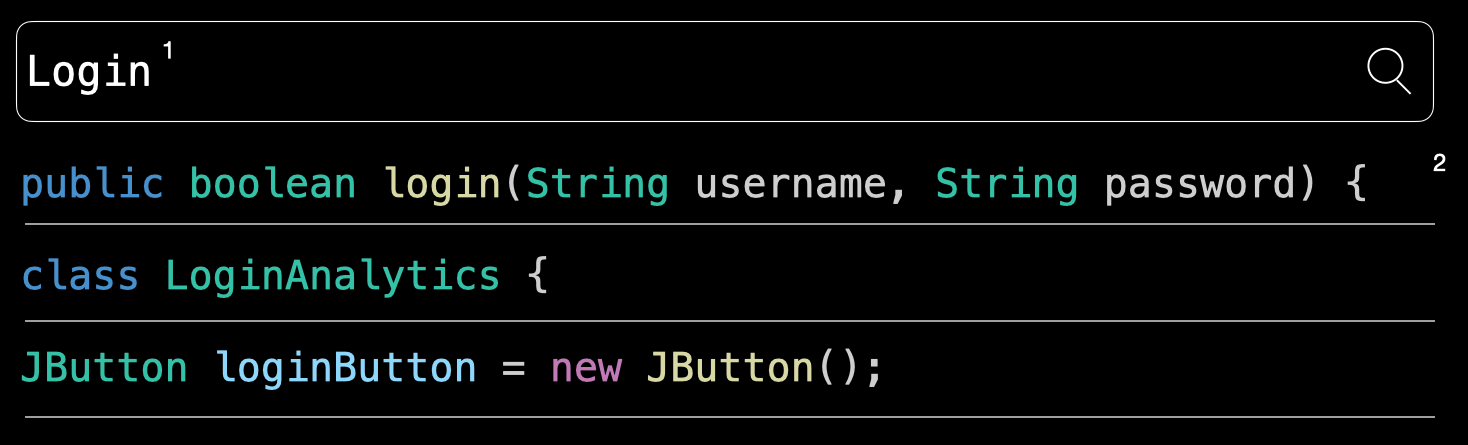
\includegraphics[width=\textwidth,keepaspectratio=true]{imagens/conceitos/code-search-structure.png}
    \smallcaption{Fonte: Autor}
    \label{fig:concepts:code-search-structure}
\end{figure}

Na Figura \ref{fig:concepts:code-search-structure}, a intenção do usuário era encontrar trechos de código-fonte relacionados a autenticação em determinado sistema. A \textit{query} utilizada para essa busca foi \textit{login} (1) e, para essa \textit{query}, foram encontrados três trechos de código-fonte (2).

Dito isso, \textcite{Grazia2022CodeSA} realizaram uma extensa revisão nos trabalhos da área e, segundo os autores, três fatores são considerados ao desenvolver sistemas de busca de código-fonte. São estes:
\begin{itemize}
  \item Facilidade de uso: o usuário deve ser capaz de criar \textit{queries} sem treinamento ou conhecimento prévio do sistema.
  \item Expressividade: dada quaisquer intenção do usuário, este deve ser capaz de expressá-la por meio de \textit{queries}.
  \item Precisão: as \textit{queries} devem ser capazes de expressar a intenção do usuário com o mínimo de ambiguidade.
\end{itemize}

\textit{Queries}, como dito anteriormente, são a interface do usuário com o sistema. Em busca de código-fonte, há diferentes formas de \textit{queries}, dependendo do sistema. 
Trabalhos como \cite{NGUYEN2017CombiningWW}, \cite{Chen2018ANF} e \cite{Du2021IsAS} utilizam \textit{queries} em linguagem natural, como português ou inglês. Este formato de \textit{queries} proporciona facilidade de uso e expressividade, enquanto perde em precisão da \textit{query} pelo fato de haver ambiguidades inerentes às linguagens naturais. Sistemas como \textit{Google}, \textit{Stack Overflow} e \textit{Github} utilizam esse formato de \textit{query}.

Outros trabalhos, como \textcite{Zhou2018SLAMPARC}, \textcite{Fujiwara2019CodetoCodeSB} e \textcite{Mukherjee2020SearchingAD}, utilizam \textit{queries} no formato de código-fonte. Uma possível \textit{query} desses sistemas seria apenas a declaração de uma função em linguagem de programação. Com isso, o sistema seria responsável por procurar trechos de código-fonte que servissem como corpo dessa função. \textit{Queries} neste formato provêm facilidade de uso, mas a precisão e expressividade variam de acordo com a intenção do usuário \cite{Grazia2022CodeSA}. Por fim, tais sistemas são utilizados, principalmente, para sugestões de código-fonte enquanto o usuário escreve o código.

\textcite{Martie2015CodeExchangeSR} e \textcite{Sivaraman2019ActiveIL} propuseram uma linguagem de busca estruturada, similar às linguagens de banco de dados como \gls{sql} para busca de código-fonte. Para encontrar códigos-fonte com os trechos \textit{import math} e \textit{def sum(a, b):}, uma possível \textit{query} válida nesses sistemas seria \textit{'import math' AND 'def sum(a,b):'}. Com essa estrutura de \textit{queries}, tais sistemas provem alta precisão e expressividade, em detrimento da facilidade de uso, pelo fato do usuário precisar aprender uma nova linguagem para realizar as buscas.

Por outro lado, trabalhos como \textcite{Reiss2009SemanticsbasedCS} e \textcite{Jiang2018ResearchPS} recebem a entrada e saída esperadas como \textit{queries}, e buscam códigos-fonte que, dada tal entrada produza a saída correspondente. Por exemplo: dada a entrada esperada 'nOmE' e a saída esperada 'nome', o sistema irá buscar códigos-fonte que produzam tal saída, dada tal entrada. Tal formato de \textit{query} provê facilidade de uso, mas são necessárias muitas \textit{queries} para se alcançar expressividade e, principalmente, precisão. Ainda, tais sistemas possuem aplicações em metodologias de desenvolvimento de \textit{software} como \textit{test-driven development}, onde o usuário primeiro escreve os testes para depois implementar a funcionalidade. A ideia é que, dado os testes (que possuem valores de entrada e saída definidos), o sistema de busca de código-fonte encontre quais trechos de código satisfazem tais testes.

Além disso, há diferentes técnicas de busca de código-fonte na literatura. Trabalhos como \textcite{Lu2015QueryEV} e \textcite{Li2016RelationshipawareCS}, por exemplo, utilizam uma técnica chamada \textit{query expansion}. Nela, dada uma \textit{query} o sistema realiza mais de uma busca com termos similares aos da \textit{query}, a fim de melhorar os resultados da busca. 

Depois, trabalhos como \textcite{Mitra2018AnIT}, \textcite{Gu2018DeepCS} e \textcite{Sun2022CodeSB} utilizam técnicas de \textit{machine learning} no problema de busca de código-fonte a partir de linguagem natural. Durante o aprendizado, estes modelos geram \textit{embeddings} para dois domínios: de linguagem natural e de código-fonte. O primeiro, geralmente são extraídos textos de comentários e documentações, os quais descrevem as tarefas realizadas por determinado código-fonte. O segundo corresponde ao código-fonte em si. Com isso, a similaridade entre a \textit{query} e o código-fonte se dá no espaço vetorial dos \textit{embeddings}.

De forma semelhante, trabalhos recentes como \textcite{Feng2020CodeBERTAP} e \textcite{Guo2021GraphCodeBERTPC} utilizam modelos \textit{transformers} para aprender as relações semânticas entre linguagem natural (da \textit{query} e das descrições dos códigos-fontes presentes nas bases de treinamento) e do código-fonte. Atualmente, tais sistemas são o estado da arte na área de busca de código-fonte.

\section{Aprendizagem de máquina em Processamento de Linguagem Natural}

A aplicação de técnicas de aprendizagem de máquina tem melhorado significativamente o estado da arte da área de processamento de linguagem natural, conforme visto em modelos como \gls{nbow}, \gls{deepcs} e \gls{bert}.

Porém, modelos de aprendizagem de máquina trabalham com números ao invés de texto. Com isso, para utilizar esses modelos dentro da área de \gls{nlp}, utiliza-se um conjunto de técnicas chamado \textit{word embedding}. Tais técnicas criam representações vetoriais a partir de \textit{tokens}, os quais podem então servir como entrada para modelos de aprendizagem de máquina. Desse conjunto de técnicas, destaca-se a família de algoritmos \textit{Word2Vec} \cite{Mikolov2013EfficientEO} \cite{Mikolov2013DistributedRO}.

Os \textit{tokens} utilizados pelo \textit{word embedding} são gerados por algoritmos chamados tokenizadores. Estes algoritmos geram \textit{tokens} a partir de determinado corpus ou bases textuais \cite{Mielke2021BetweenWA}. \textit{Tokens} são unidades menores dos textos, como por exemplo palavras, morfemas ou símbolos específicos do \textit{tokenizador} - portanto, os \textit{tokens} gerados dependem do tokenizador. Em modelos \textit{transformers}, os tokenizadores mais utilizados são \gls{bpe} e \textit{WordPiece}.

O \gls{bpe} inicialmente cria uma lista com todas as palavras distintas do corpus de treinamento. A partir dessa lista, um vocabulário é gerado com todas as letras distintas - e textos com palavras que não estavam no corpus de treinamento serão substituídos pelo token \textit{unknown} (desconhecido). Aqui, vale ressaltar que modelos transformers como \gls{gpt2} e \gls{roberta} utilizam uma variação do \gls{bpe} chamada \textit{byte-level} \gls{bpe}, a qual utiliza \textit{bytes} ao invés das letras em formato Unicode, eliminando assim a necessidade do \textit{token} '\textit{unknown}'.

A partir do vocabulário inicial, o \gls{bpe} itera sobre todo o corpus de treinamento para determinar a frequência com que os \textit{tokens} de seu vocabulário ocorrem. Então, são gerados pares (daí o nome \textit{byte-pair}) contendo o \textit{token} e sua frequência no corpus de treinamento. Ao fim, o \gls{bpe} concatena os dois \textit{tokens} dos pares mais frequentes nessa iteração, a fim de criar um novo \textit{token} em seu vocabulário. Tais relações entre \textit{tokens}, aprendidas a partir de suas frequências no corpus de treinamento, são chamadas de regras de \textit{merge}. Por fim, vale notar que, a cada iteração, é adicionado um novo \textit{token} ao vocabulário do tokenizador. E a a quantidade de iterações que o tokenizador fará, e portanto o tamanho de seu vocabulário, é determinada pelo usuário.

O \textit{WordPiece} segue praticamente os mesmos passos do \gls{bpe}, com algumas diferenças da implementação. Inicialmente, o \textit{WordPiece} também gera um vocabulário a partir das palavras distintas que ocorrem no corpus de treinamento. A diferença em relação ao \gls{bpe} é que o \textit{WordPiece} adiciona um prefixo que indica a continuação de determinada palavra, às letras do vocabulário. Por exemplo, dada a palavra $frase$, os seguintes \textit{tokens} serão gerados: $[f, \#\#r, \#\#a, \#\#s, \#\#e]$. Outra diferença em relação ao \gls{bpe} é que, ao invés da frequência, os \textit{tokens} são combinados utilizando uma nota dada pelo \textit{WordPiece} a cada \textit{token}. Essa nota é computada utilizando a seguinte equação:
\begin{equation*}
y=\frac{f_{1,2}}{f_1 \times f_2}
\end{equation*}
Na equação acima, $y$ é a nota do \textit{token}, $f_{1,2}$ é a frequência do par de \textit{tokens}, $f_1$ a frequência do o primeiro \textit{token} do par e $f_2$ do segundo \textit{token}. Com isso, são gerados os \textit{tokens} de determinado corpus.

\section{Modelos de Atenção}
Modelos \textit{transformers}, como \gls{bert} e \gls{roberta}, utilizam algum tipo de modelo de atenção (ou mecanismo de atenção). Segundo \textcite{Vaswani2017AttentionIA}, atenção pode ser descrita como uma função de mapeamento entre um vetor \textit{query} $Q$ e um par chave-valor de vetores $K$ e $V$, respectivamente. \textcite{Vaswani2017AttentionIA} propõe uma função de atenção, chamada \textit{Scaled Dot-Product Attention}, a qual é descrita da seguinte forma \cite{Vaswani2017AttentionIA}:
\begin{equation*}
A(Q, K, V)= softmax(\frac{QK^T}{\sqrt{d_k}}) \times V
\label{eq:attention-equation}
\end{equation*}
Na qual $d_k$ é a dimensão do vetor $K$. Como o resultado do $softmax$ consiste em uma distribuição de probabilidades, a multiplicação vetorial do vetor resultante de $softmax(\frac{QK^T}{\sqrt{d_k}})$ com o vetor $V$ ativará alguma dimensão de $V$, indicando assim a atenção de $Q$ e $K$ em $V$, ou $A(Q, K, V)$.

Além disso, os modelos \textit{transformers} utilizam uma técnica chamada \textit{multi-head attention}. Nela, são realizadas projeções lineares dos vetores $Q$, $K$ e $V$, as quais foram aprendidas durante a fase de treinamento \cite{Vaswani2017AttentionIA}. Isso permite com que o modelo consiga observar, de forma conjunta, diferentes representações de determinado \textit{token} em diferentes posições do texto.

A arquitetura \textit{transformer} também prevê um vetor de posição para cada \textit{token}, para descrever sua posição no texto. Esse vetor é chamado \textit{positional encoding} e foi descrito por \textcite{Vaswani2017AttentionIA} da seguinte forma:
\begin{eqnarray*}
PE_{(pos, 2_i)} & = &\sin{\frac{pos}{10000^\frac{2_i}{d_m}}} \\
PE_{(pos, 2_(i+1))} & = & \cos{\frac{pos}{10000^\frac{2_i}{d_m}}}
\end{eqnarray*}
Na equação acima, $pos$ é a posição do \textit{token}, $d_m$ é a dimensão do modelo e $i$ é a dimensão atual, sendo que $0 \leq i \leq d$. Como as funções de seno e cosseno são periódicas, os valores gerados estarão entre $2\pi$ e $10000 \times 2\pi$. Com isso, o \textit{positional encoding} é capaz de descrever as posições absolutas e relativas de determinado \textit{token} no texto. Vale frisar que é possível descrever posições relativas neste modelo pois, dado um intervalo $k$ entre um \textit{token} e outro \textit{token} anterior, $PE_{pos+k}$ pode ser representado como função linear de $PE_{pos}$ \cite{Vaswani2017AttentionIA}.

Por fim, a Figura \ref{fig:transformer-architecture} mostra um diagrama com uma visão geral da arquitetura \textit{transformer}:

\begin{figure}[H]
    \centering
    \caption{Visão geral da arquitetura \textit{Transformer}}
    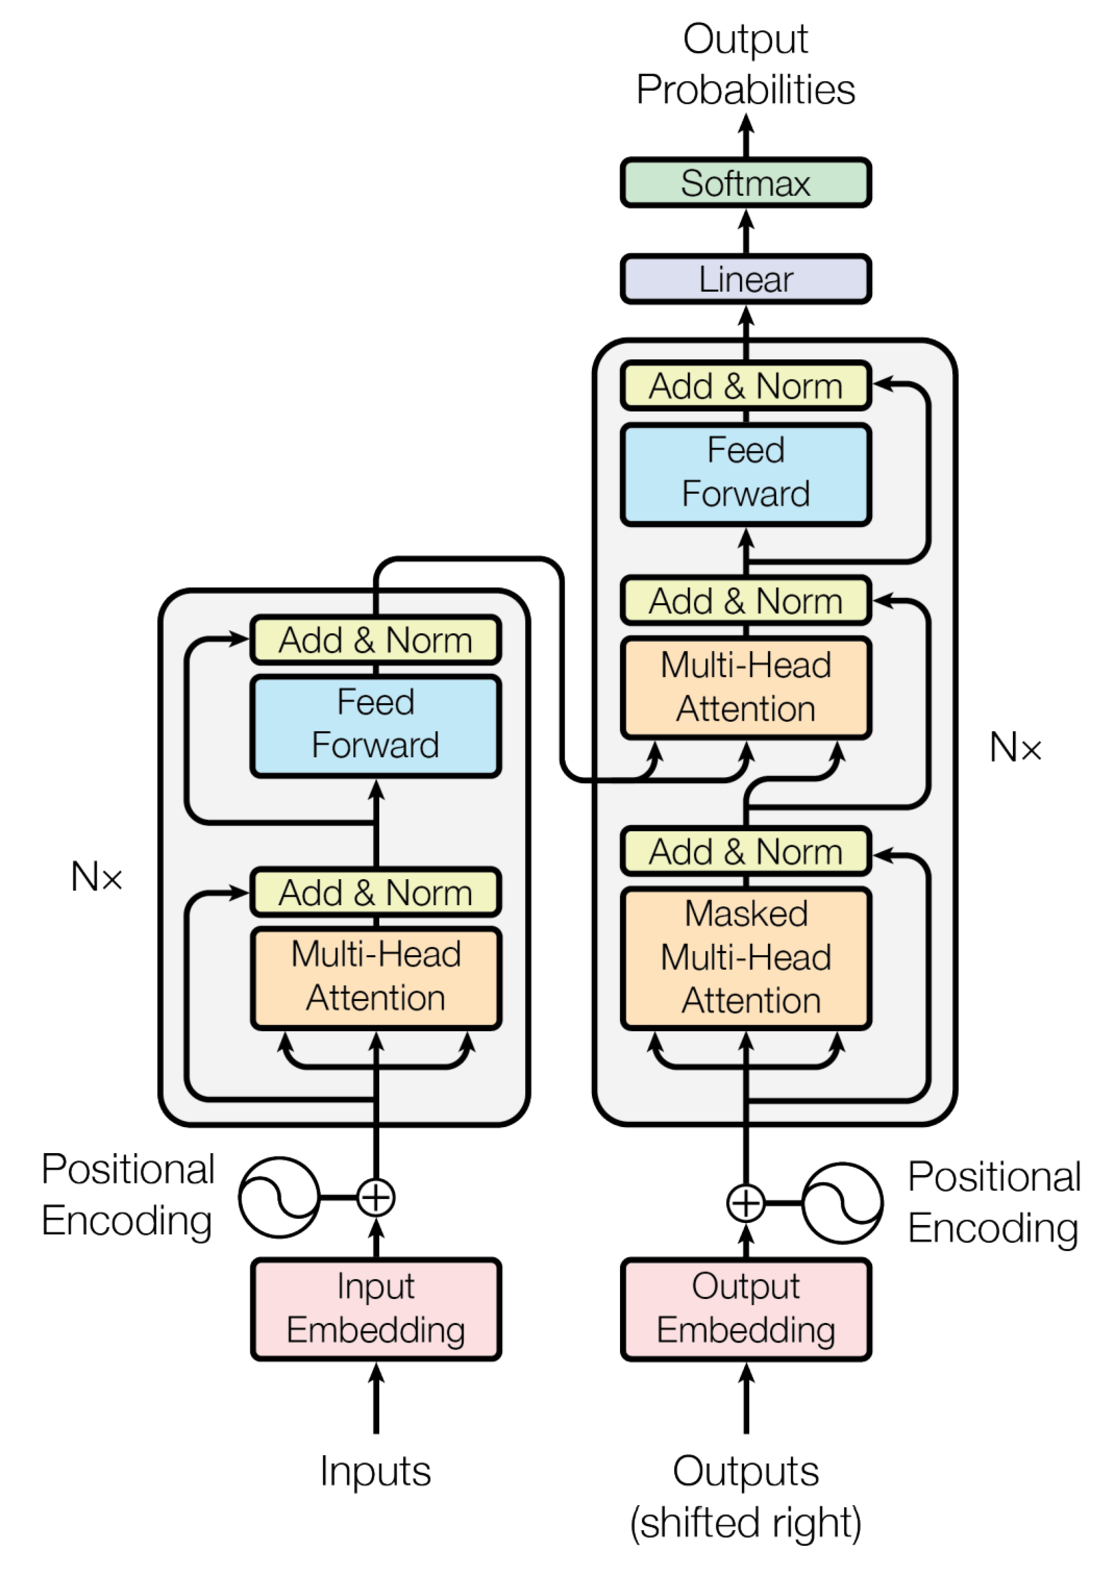
\includegraphics[scale=0.4]{imagens/conceitos/transformer-architecture.pdf}
    \smallcaption{Fonte: \cite{Vaswani2017AttentionIA}}
    \label{fig:transformer-architecture}
\end{figure}

Vale ressaltar que o \textit{pipeline} do lado esquerdo da Figura \ref{fig:transformer-architecture}, o qual recebe os \textit{embeddings} de entrada (\textit{input embeddings)}, é chamado de \textit{encoder}. E o \textit{pipeline} do lado direto da Figura \ref{fig:transformer-architecture} é chamado de \textit{decoder}.

Posteriormente, foi proposto o modelo \gls{bert} \cite{Devlin2019BERTPO}. Este consegue aprender, dado um \textit{token} do texto, o contexto tanto com os \textit{tokens} anteriores quanto com seus sucessores. Em outras palavras, o \gls{bert} aprende o contexto de forma bi-direcional. Como exemplo, dada a sentença "O menino foi passear na praia", modelos anteriores ao \gls{bert} processavam as palavras em sequência - primeiro "O", depois "menino", depois "foi" e assim por diante - até por conta dessa limitação que modelos como \gls{lstm} eram recursivos, a fim de guardar as informações de palavras previamente processadas; no exemplo em questão, para saber o contexto ao processar a palavra "foi", era necessário que estes modelos recorrentes salvassem as informações obtidas das palavras anteriores "O" e "menino".

Ainda, como o \gls{bert} utiliza apenas modelos de atenção, este consegue processar todas as palavras da frase em paralelo, aumentando drasticamente a performance de treinamento em relação aos modelos recorrentes, por exemplo. Porém, só os modelos de atenção não seriam suficientes para possibilitar o processamento em paralelo das palavras durante o treinamento do \gls{bert}, já que as posições das palavras na frase seriam perdidas. Por isso, além dos modelos de atenção, os modelos \textit{transformers} e, mais especificamente, o \gls{bert}, utilizam os \textit{positional embeddings} citados acima. Estes vetores descrevem tanto as posições relativas quanto absolutas de cada palavra na frase. Para fins didáticos, e utilizando a mesma frase "O menino foi passear na praia", considere que cada palavra é numerada a partir de zero - então, "O" estaria na posição 0, "menino" na posição 1 e assim por diante. Nesse caso, a posição absoluta da palavra "passear" seria 3 e a posição relativa à palavra "O" seria 2.

Além disso, também é possível pré treinar os modelos \textit{transformers}. Como tais modelos demandam muitos recursos computacionais durante seu treinamento, estes são geralmente pré-treinados com grandes quantidades de dados \textit{corpus} grande em determinado domínio. Por exemplo, dado o par código-fonte/comentário, tem-se dois domínios diferentes: código-fonte e linguagem natural, respectivamente. Portanto, utilizou-se dois modelos \textit{transformers} - um pré treinado com amostras de código-fonte, e outro com trechos de textos na lingua inglesa, conforme descrito no capítulo \ref{chp:experiments}. Com isso, não foi necessário treinar tais modelos de \textit{embedding} com a base de dados específica utilizada no presente estudo. 

Entretanto, é possível especializar ainda mais os modelos \textit{transformers} utilizando um processo chamado \textit{fine-tuning} onde, dado um domínio específico (como busca de código-fonte a partir de linguagem natural), tais modelos são treinados utilizando amostras específicas para o problema em questão, a fim de especializar os modelos \textit{transformers} no problema em questão e, com isso, aumentar sua performance. Como tal processo demanda muitos recursos, além de fugir do objetivo principal do presente estudo, o \textit{fine-tuning} não foi realizado para nenhum dos modelos \textit{transformers} citados no capítulo \ref{chp:experiments} \cite{Tay2021ScaleEI}.

\section{Métricas de Avaliação de Recuperação de Informação}
Dado uma lista de resultados para determinada busca, ordenados de maneira decrescente de relevância, o \gls{mrr} é um valor, entre 0 e 1, que representa em qual posição o resultado mais relevante estará na lista de resultados. Caso o \gls{mrr} seja 1, o resultado mais relevante estará (na maioria dos casos) em primeiro lugar na lista de resultados; se for 0.5, este estará na segunda posição e assim por diante \cite{Craswell2009}. Essa métrica é composta pela a média entre os resultados de várias buscas em determinada base de dados. Os valores individuais de cada busca são chamados de \gls{rr} e são calculados da seguinte forma:
\begin{equation*}
    RR_i=1/rank_i
\end{equation*}
Na equação acima, $rank_i$ é a posição de determinado resultado - se este estiver na primeiro posição, $RR=1/1=1$; se estiver na segunda, $RR=1/2=0.5$ e assim por diante. Com isso, tem-se que o \gls{mrr} é a média harmônica de todos os \glspl{rr} para a quantidade de buscas realizadas em determinada base de dados. Portanto, a fórmula do \gls{mrr} é dada por:
\begin{equation*}
    MRR = \frac{1}{|Q|} \times \sum_{i=1}^{|Q|} RR_i
\end{equation*}
Na qual $|Q|$ é a quantidade de buscas realizadas.

Por sua vez, \textit{SuccessRate@k} é um valor, entre 0 e 1, que representa a porcentagem de vezes que o resultado mais relevante da busca esteve nas primeiras $k$ posições da lista de resultados. Essa métrica é descrita pela fórmula \cite{Wan2019MultimodalAN}:
\begin{equation*}
    SuccessRate@k=\frac{1}{|Q|} \times \sum_{i=1}^{|Q|} \delta(FRank_i \geq k)
\end{equation*}
Na qual $\delta(x)$ é uma função que retorna 1 caso x for verdadeiro e 0 caso contrário. $FRank_i$ é a posição do resultado relevante na lista de resultados \cite{Raghothaman2016SWIMSW}. Por fim, vale ressaltar que autores tem utilizado outros nomes para se referir à essa mesma métrica. Citando alguns exemplos, \textcite{Ling2020AdaptiveDC} se refere à essa métrica como \textit{Hit@k}, \textcite{Bui2021SelfSupervisedCL} como \textit{Precision@k} e, ainda, \textcite{Gu2021CRaDLeDC} como \textit{R@k}. No presente estudo, entretanto, essa métrica será chamada de \textit{SuccessRate@k}.

